\documentclass[a4paper,french]{article}
\usepackage[utf8]{inputenc}
\usepackage[francais]{babel}
\usepackage[babel=true]{csquotes}
\usepackage{graphicx}

\pagestyle{headings}

\title{Structure des ordinateurs : Projet 2}
\author{Raphaël Javaux}
\date{}

\begin{document}

\maketitle

\section{Introduction}

    \paragraph{} Notre algorithme de génération aléatoire de labyrinthes utilise
une structure de données efficace pour stocker l'état du labyrinthe et de ses
murs ainsi que pour effectuer les regroupements des cellules lorsqu'un mur est
supprimé.
    \newline Cette structure, nommée \textit{Union-find}, est décrite en détail
sur l'article correspondant de Wikipedia
\footnote{http://fr.wikipedia.org/wiki/Union-Find}. Le regroupement de deux
cellules se fait en parallèle si au moins l'une de ces deux-ci ne se trouve pas
dans un groupes de cellules dont certaines sont partagées par un autre
processus.
    \newline Contrairement à un algorithme de remplissage plus naïf, notre
algorithme effectue les regroupement en temps constant \underline{sans}
augmenter l'espace mémoire nécessaire par rapport à ces premiers algorithmes.

\section{Structure des données}
\label{donnees}

    \paragraph{} L'ensemble des cellules du labyrinthe sont stockées dans un
même vecteur.
    \newline Chaque cellule est stockée dans un entier non signé de 16 bits. Les
quatre premiers bits encodent les états des quatre murs de la cellule. Le bit
suivant définit si cette cellule est partagée entre plusieurs processus (voir
section \ref{parallelisme}). Les onze derniers bits encodent l'indice de la
cellule parente dans le vecteur des cellules, de telle manière à aboutir à la
structure hiérarchique \textit{Union-find}.

    \paragraph{} Lorsque l'indice du parent est identique à l'indice de la
cellule, alors celle-ci est sa propre parente.
    \newline Chaque cellule appartient à un groupe (l'ensemble des cellules
accessibles à partir de cette cellule) et ce groupe est identifié de manière
unique par sa racine, c'est à dire la première cellule étant sa propre parente
lorsque l'on remonte l'arbre dessiné par les indices des parents.

    \paragraph{} Avec cette structure, la fusion de deux groupes peut se faire
très aisément : il suffit de modifier l'indice du parent de la racine du premier
groupe pour qu'il pointe vers une cellule quelconque du second groupe :

    \begin{center}
        \includegraphics{schema_fusion.eps}
    \end{center}

    \paragraph{} Pour éviter que l'arbre ne gagne trop en profondeur, une
procédure aplatit partiellement l'arbre à chaque recherche de la racine d'une 
cellule, comme cela est décrit sur l'article de Wikipedia.

    \paragraph{} Avec cette méthode, les opérations de suppression des murs se
font en temps algorithmique quasiment constant, au contraire d'un algorithme de
remplissage qui est linéaire en temps par rapport au nombre de cellules des
deux groupes à fusionner, tout en occupant rigoureusement le même espace mémoire
(les numéros des couleurs du graphe sont remplacés par les indices des parents).

\section{Implémentation parallèle}
\label{parallelisme}

    \paragraph{} Le principal problème auquel une implémentation concurrente
de l'algorithme doit répondre est de garantir l'intégrité des labyrinthes
générés.
    \newline En particulier, il convient d'éviter que deux processus distincts
suppriment deux murs (distincts ou non) départageant deux même groupes au même
moment.

    \paragraph{} Sur le dessin suivant, les deux murs en bleu ne peuvent en aucun
cas être supprimés en même temps par les deux différents processus car cela
créerait deux chemins différents liant deux mêmes cellules, et le labyrinthe ne
serait plus parfait. Les lignes rouges représentent les séparations entre les
quatre processus générateurs.

    \begin{center}
        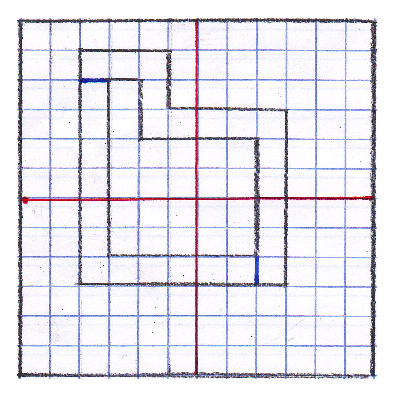
\includegraphics{schema_conflit.eps}
    \end{center}

    \paragraph{} Notre approche pour résoudre ces conflits est d'acquérir un
verrou exclusif sur l'ensemble de la grille pour supprimer un mur si et
seulement si ce dernier sépare deux groupes de cellules partagés entre plusieurs
processus.

    \paragraph{} En effet, lors de la suppression d'un mur, trois cas peuvent se
produire :

    \begin{itemize}
        \item Le mur sépare deux groupes non partagés. Il n'y a dans ce cas
aucun conflit et la fusion se faire en parallèle sans verrou ;
        \item Le mur sépare deux groupes partagés par plusieurs processus.
Dans ce cas, il faut impérativement bloquer l'ensemble des autres processus ;
        \item Le mur sépare un groupe partagé et un groupe non partagé. Il n'est
pas nécessaire d'acquérir un verrou si l'on ne modifie pas le groupe partagé.
Nous effectuons donc la fusion en modifiant la racine du groupe non partagé pour
que celle-ci pointe vers une cellule du groupe partagé.\footnote{Avec un
algorithme de remplissage, nous remplirions les cellules du groupe non partagé
de la couleur du groupe partagé.}
    \end{itemize}

    \paragraph{} Comme expliqué au cours de la section \ref{donnees}, chaque
cellule contient un bit indiquant si cette dernière est partagée ou non, c'est à
dire si son groupe peut être modifié par plusieurs processus ou non.
    \newline Les cellules partagées sont grisées sur le schéma suivant. Il 
s'agit des cellules dont au moins l'un des murs peut être détruit par plusieurs
processus.

    \begin{center}
        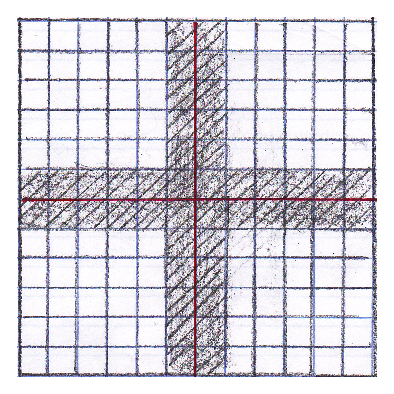
\includegraphics{schema_partages.eps}
    \end{center}

    \paragraph{} Etant donné que la fusion de deux groupes se fait toujours en
sélectionnant le ou l'un des groupes partagés comme nouvelle racine si au moins
l'un de ces deux-ci est partagé, un groupe dont au moins une de ses cellules
est partagée aura toujours une cellule partagée comme racine. Nous utilisons
donc le bit de partage de la racine d'un groupe pour savoir si celui-ci est
partagé entre plusieurs processus.

    \paragraph{} Chaque processus générateur continue de supprimer des murs tant
que l'ensemble de ses cellules ne fait pas partie du même groupe.

\section{Performances}

    \paragraph{} Pour mesurer les performances de notre algorithme, nous avons
mesuré le nombre total de suppressions de murs s'étant effectuées sans garder un
verrou exclusif sur l'ensemble de la grille par rapport au nombre total de murs
qui ont été supprimés.

    \paragraph{} Etant donné que le nombre de cellules partagées augmente moins
rapidement que le nombre total de cellules du labyrinthe lorsque l'on augmente
la taille du labyrinthe, les performances de la parallélisation sont bien plus
importantes lorsque le labyrinthe est de grande taille.

    \paragraph{} Dans le cas d'un labyrinthe de 12 cases de large, 69\% des
suppressions des murs se font en moyenne en parallèle. Avec 42 cases de large,
plus de 90\% des suppressions sont effectuées sans le verrou global.

    \begin{center}
        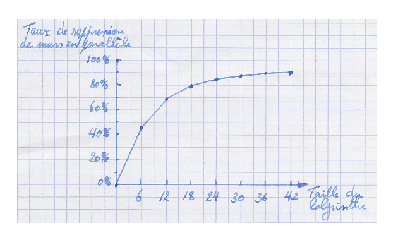
\includegraphics{schema_performances.eps}
    \end{center}

    \paragraph{} 



\end{document}